\documentclass{article}

\usepackage{graphicx}
\usepackage{tikz}
\usepackage{tikzsymbols}
\usetikzlibrary{calc,patterns,shapes.geometric}
\pagestyle{empty}
\usepackage[margin=0pt]{geometry}
\geometry{papersize={14in,12in}}

\def\centerarc[#1](#2)(#3:#4:#5){\draw[#1] ($(#2)+({#5*cos(#3)},{#5*sin(#3)})$) arc (#3:#4:#5);}

\begin{document}
	\begin{figure}
		\centering
		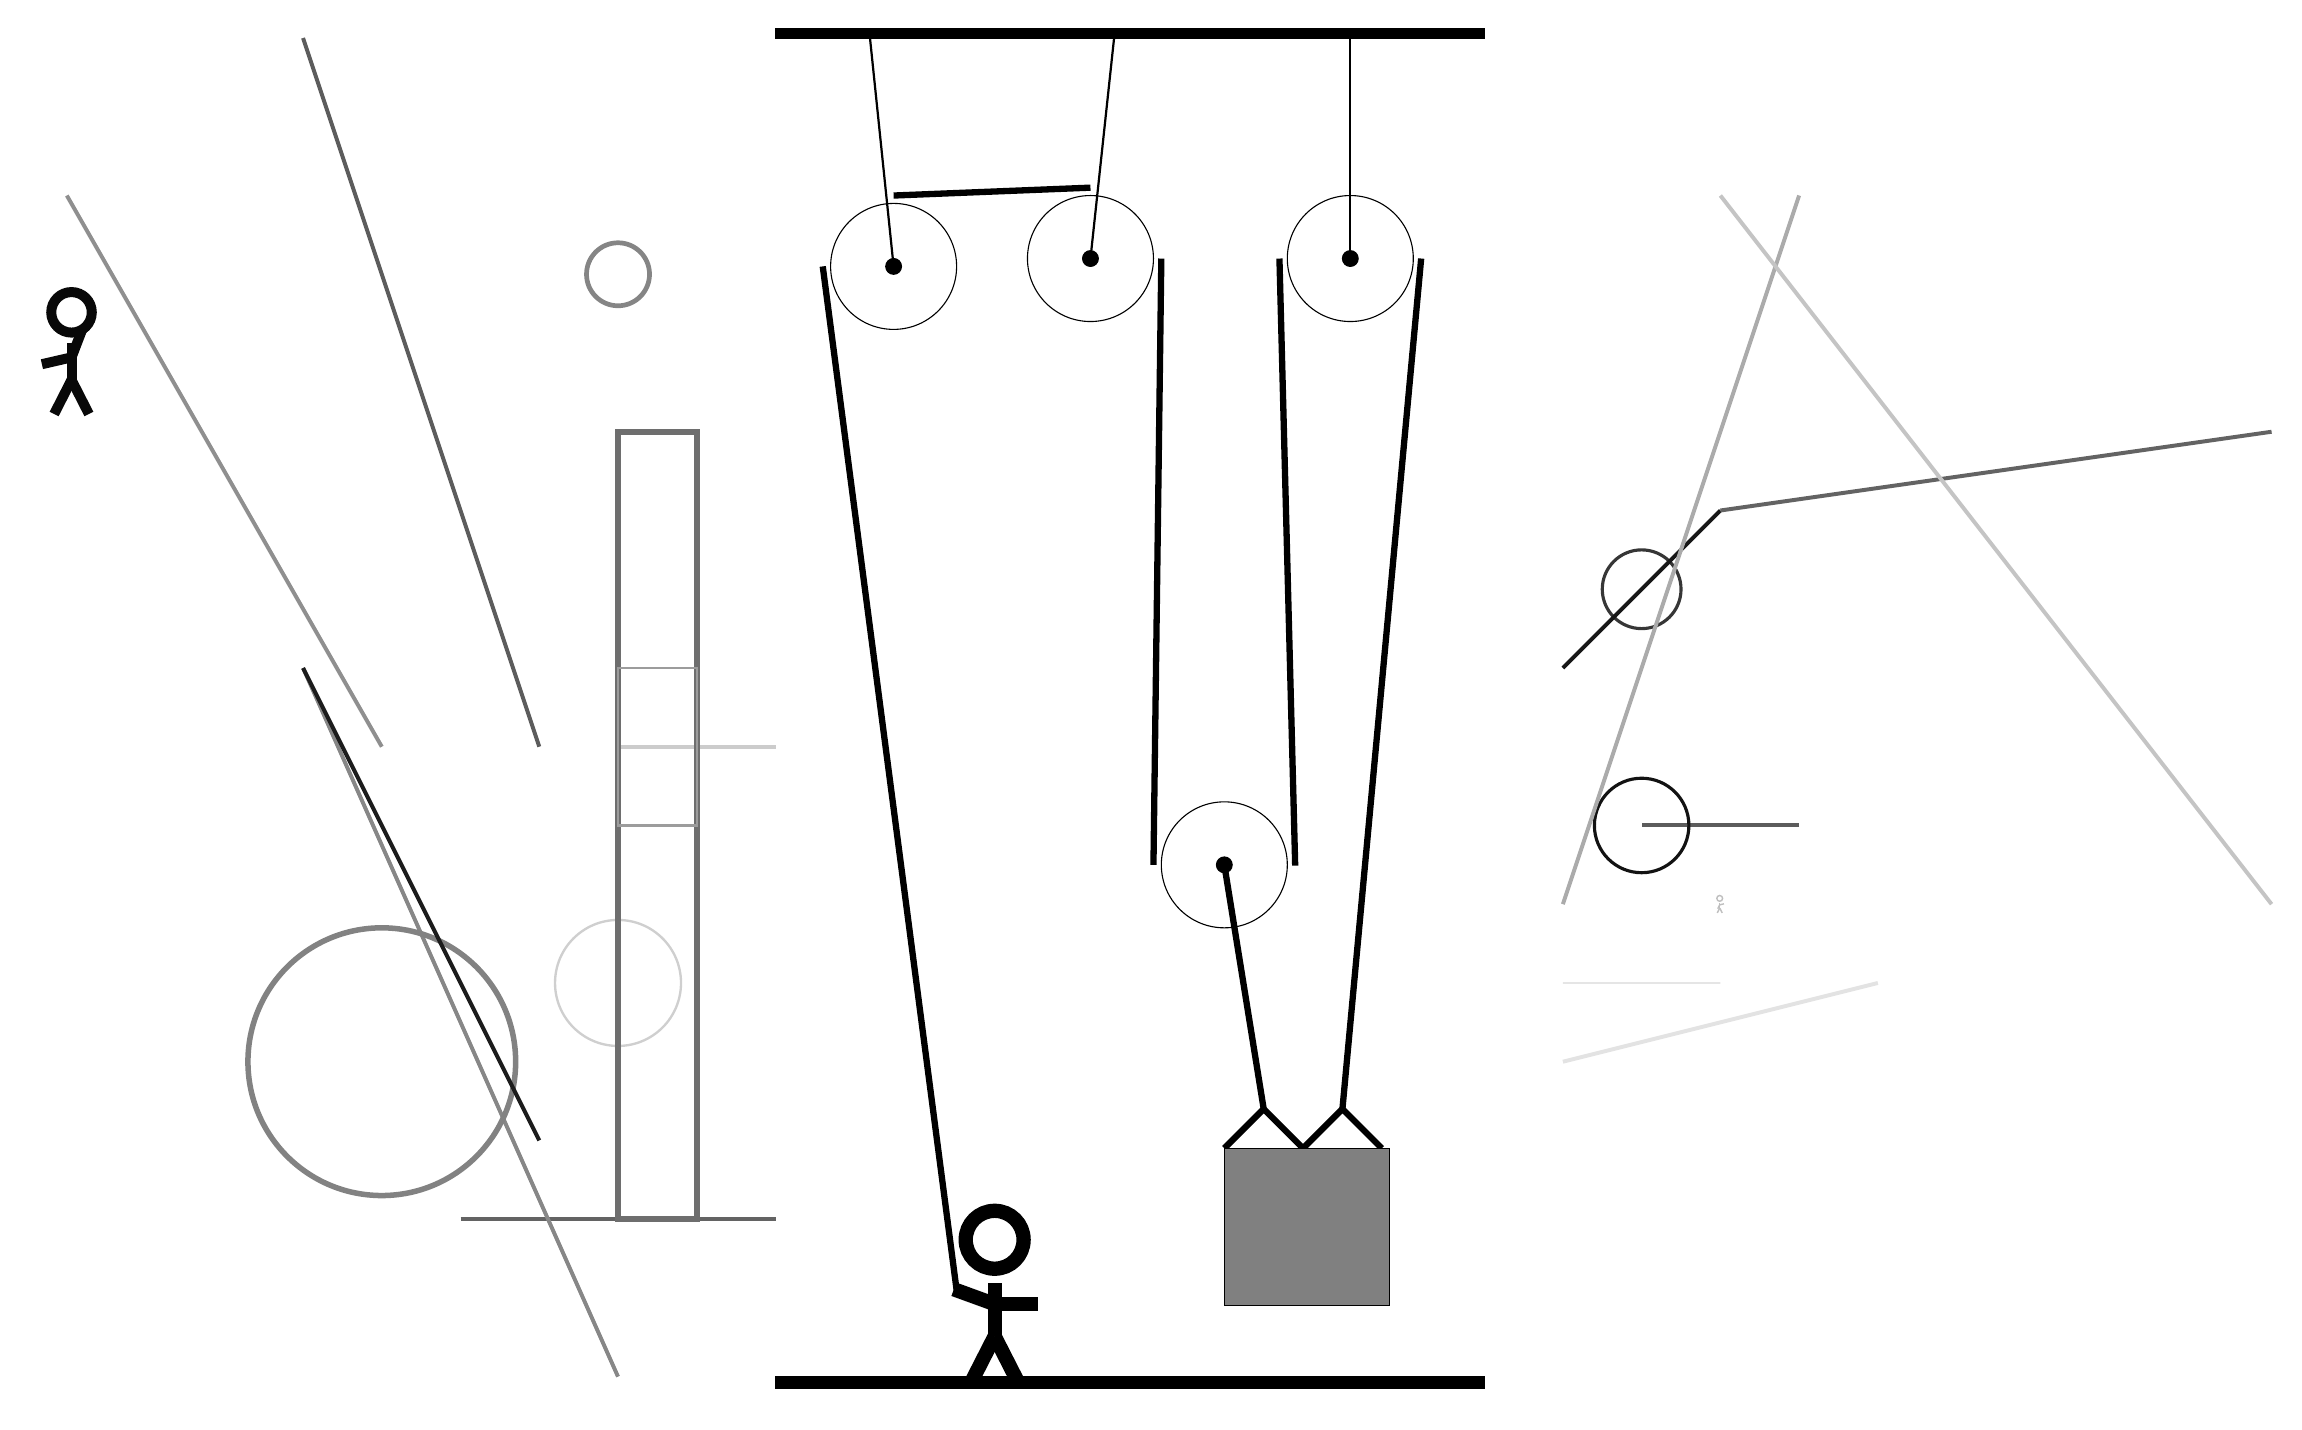
\begin{tikzpicture}
			%%%%% START %%%%%
			
			\draw[fill=black] (-3, 14) rectangle (6, 14.125);
			
			\draw (1, 11.2) circle (0.8);
			\draw[fill=black] (1, 11.2) circle (0.1);
			\draw[thick] (1, 11.2) -- (1.3, 14);
			
			\draw (4.3, 11.2) circle (0.8);
			\draw[fill=black] (4.3, 11.2) circle (0.1);
			\draw[thick] (4.3, 11.2) -- (4.3, 14);
			
			\draw[line width=0.5mm, color=black!61](-7, -1) -- (-3, -1);
			
			\draw [line width=0.3mm, color=black!19](-5, 2) circle (0.8);
			\draw [line width=0.4mm, color=black!79](8, 7) circle (0.5);
			\draw[line width=0.5mm, color=black!91](9, 8) -- (7, 6);
			\draw[line width=0.5mm, color=black!20](-3, 5) -- (-5, 5);
			
			\draw[line width=0.3mm, color=black!10] (7, 2) rectangle (9, 2);
			\draw[line width=0.5mm, color=black!11](7, 1) -- (11, 2);
			\node[line width=0.6mm, color=black!25] at (9, 3) {\Strichmaxerl[1][63][13]};
			\draw[line width=0.5mm, color=black!64](-6, 5) -- (-9, 14);
			\draw[line width=0.5mm, color=black!64](10, 4) -- (8, 4);
			
			\draw [line width=0.4mm, color=black!93](8, 4) circle (0.6);
			
			\draw[line width=0.7mm, color=black!57] (-5, -1) rectangle (-4, 9);
			\draw[line width=0.5mm, color=black!47](-5, -3) -- (-9, 6);
			
			\node[line width=0.7mm, color=black!97] at (-12, 10) {\Strichmaxerl[7][13][69]};
			\draw [line width=0.7mm, color=black!49](-8, 1) circle (1.7);
			\draw [line width=0.6mm, color=black!48](-5, 11) circle (0.4);
			
			\draw[line width=0.3mm, color=black!39] (-4, 4) rectangle (-5, 6);
			\draw[line width=0.5mm, color=black!33](7, 3) -- (10, 12);
			\draw[line width=0.5mm, color=black!61](9, 8) -- (16, 9);
			
			\draw[line width=0.5mm, color=black!89](-6, 0) -- (-9, 6);
			\draw[line width=0.5mm, color=black!23](9, 12) -- (16, 3);
			
			\draw [line width=0.2mm, color=black!86](-6, 14) circle (0.0);
			\draw[line width=0.5mm, color=black!44](-8, 5) -- (-12, 12);
			
			\draw (2.7, 3.5) circle (0.8);
			\draw[fill=black] (2.7, 3.5) circle (0.1);
			
			\draw[line width=0.8mm]  (2.7, -0.1) -- (3.2, 0.4) -- (3.7, -0.1) -- (4.2, 0.4) -- (4.7, -0.1);
			\draw[fill=black!50] (2.7, -0.1) rectangle (4.8, -2.1);
			
			\draw (-1.5, 11.1) circle (0.8);
			\draw[fill=black] (-1.5, 11.1) circle (0.1);
			\draw[thick] (-1.5, 11.1) -- (-1.8, 14);
			
			\draw[line width=0.8mm](-0.7, -1.9) --  (-2.4, 11.1);
			\centerarc[line width=0.8mm](-1.5, 11.1)(90:180:0.9);
			\draw[line width=0.8mm](-1.5, 12.0) -- (1, 12.1);
			\centerarc[line width=0.8mm](1, 11.2)(0:90:0.9);
			\draw[line width=0.8mm](1.9, 11.2) -- (1.8, 3.5);
			\centerarc[line width=0.8mm](2.7, 3.5)(180:370:0.9);
			\draw[line width=0.8mm] (3.6, 3.49) -- (3.4, 11.2);
			\centerarc[line width=0.8mm](4.3, 11.2)(0:180:0.9);
			\draw[line width=0.8mm](4.2, 0.4) -- (5.2, 11.2);
			\draw[line width=0.8mm] (3.2, 0.4) -- (2.7, 3.5);
			
			\node at (-0.2, -2) {\Strichmaxerl[10][-20][0]};
			
			\draw[fill=black] (-3, -3) rectangle (6, -3.15);
			
			%%%%% END %%%%%
		\end{tikzpicture}
	\end{figure}	
\end{document}